\providecommand{\econtexRoot}{}
\renewcommand{\econtexRoot}{..}
\providecommand{\econtexPaths}{}\renewcommand{\econtexPaths}{\econtexRoot/Resources/econtexPaths}
% The \commands below are required to allow sharing of the same base code via Github between TeXLive on a local machine and Overleaf (which is a proxy for "a standard distribution of LaTeX").  This is an ugly solution to the requirement that custom LaTeX packages be accessible, and that Overleaf prohibits symbolic links
\providecommand{\econtex}{\econtexRoot/Resources/texmf-local/tex/latex/econtex}
\providecommand{\econtexSetup}{\econtexRoot/Resources/texmf-local/tex/latex/econtexSetup}
\providecommand{\econtexShortcuts}{\econtexRoot/Resources/texmf-local/tex/latex/econtexShortcuts}
\providecommand{\econtexBibMake}{\econtexRoot/Resources/texmf-local/tex/latex/econtexBibMake}
\providecommand{\econtexBibStyle}{\econtexRoot/Resources/texmf-local/bibtex/bst/econtex}
\providecommand{\econtexBib}{economics}
\providecommand{\notes}{\econtexRoot/Resources/texmf-local/tex/latex/handout}
\providecommand{\handoutSetup}{\econtexRoot/Resources/texmf-local/tex/latex/handoutSetup}
\providecommand{\handoutShortcuts}{\econtexRoot/Resources/texmf-local/tex/latex/handoutShortcuts}
\providecommand{\handoutBibMake}{\econtexRoot/Resources/texmf-local/tex/latex/handoutBibMake}
\providecommand{\handoutBibStyle}{\econtexRoot/Resources/texmf-local/bibtex/bst/handout}

\providecommand{\FigDir}{\econtexRoot/Figures}
\providecommand{\CodeDir}{\econtexRoot/Code}
\providecommand{\DataDir}{\econtexRoot/Data}
\providecommand{\SlideDir}{\econtexRoot/Slides}
\providecommand{\TableDir}{\econtexRoot/Tables}
\providecommand{\ApndxDir}{\econtexRoot/Appendices}

\providecommand{\ResourcesDir}{\econtexRoot/Resources}
\providecommand{\rootFromOut}{..} % Path back to root directory from output-directory
\providecommand{\LaTeXGenerated}{\econtexRoot/LaTeX} % Put generated files in subdirectory
\providecommand{\econtexPaths}{\econtexRoot/Resources/econtexPaths}
\providecommand{\LaTeXInputs}{\econtexRoot/Resources/LaTeXInputs}
\providecommand{\LtxDir}{LaTeX/}
\providecommand{\EqDir}{Equations} % Put generated files in subdirectory

\documentclass[pdflatex]{beamer}
\providecommand{\texname}{ProjectGAZ-Slides}% Indicate the keyname for the bibtex entry corresponding to this document
\providecommand{\texnameMaster}{ProjectGAZ}% Indicate the keyname for the bibtex entry corresponding to this document
\newif\ifdvi\dvifalse

%\usepackage{optional}
\usepackage{ifthen}%\usepackage{\econtexRoot/BufferStockTeory}

% Can't read in ProjectGAZ.sty because some packages conflict with Beamer
% So need to redefine everything here

\usepackage{\econtexShortcuts} 
\usepackage{natbib,amsmath,amssymb,rotating,subfigure}
\usepackage{verbatim,moreverb,graphicx}
\usepackage{wasysym}
\usepackage{dcolumn}
\usepackage{cancel}
\usepackage{booktabs}
%\providecommand{\LtxDir\EqDir}{\econtexRoot/Equations}
\providecommand{\FigsRaw}{\econtexRoot/Code/Python/Figures}
\providecommand{\CodeDir}{\econtexRoot/Code}
\providecommand{\CalibrationDir}{\econtexRoot/Calibration}
\providecommand{\TableDir}{\econtexRoot/Tables}
\providecommand{\ApndxDir}{\econtexRoot/Appendices}
\providecommand{\Ex}{\mathbb{E}}

%\usepackage{natbib}\newcommand*{\newblock}{}

\mode<presentation>
{
  \usetheme{Warsaw}
  % or ...
  \setbeamercovered{transparent}
}

%\beamerdefaultoverlayspecification{<+->}

%\setbeamertemplate{navigation symbols}{}  % Take away navigation symbols

\usetheme{Warsaw}

\setbeamersize{text margin left=3mm}
\setbeamersize{text margin right=3mm}


%_____________ Opening slide _______________________

\title[Sequential Bargaining]{Sequential Vote Buying with Heterogeneous Agents}
\author[Gao]{Zejun(Alice) Gao}
\institute[JHU]{Johns Hopkins University}
\date[\today]{December 21, 2021}

\begin{document}\bibliographystyle{\econtexBibStyle}

\begin{frame}[plain]
  \titlepage
\end{frame}


%_____________ 1st section  ____________
\section{Introduction}
\subsection{Motivation}

\begin{frame}
\frametitle{Motivation}
	\begin{itemize}
		\item Vote buying is a prevailing phenomenon, where political leaders offer side payments or other forms of benefits to voters or voting coalitions (like voting blocks) to gain support for a candidate or the passing of policies.
		\item The model that fits best with such scenario is sequential bargaining, where a principal negotiates with a group of n agents sequentially, and needs q agents' cooperation ($q \leq N$) to "win". For simplicity, we only consider the case with one political leader and multiple voters to avoid competition between various vote buyers.
	\end{itemize}
\end{frame}

\subsection{The Problem}
\begin{frame}
\frametitle{Key issue}
	\begin{itemize}
		\item The main problem to solve is in what order should the vote buyer approach a sequence of vote sellers (if applicable), and what offer should they make to each seller.
		\item Inspired by \cite{Cai03}, the three papers, \cite{Xiao}, \cite{InOCoHoldUP}, and \cite{CnZSeqVB}, provide different results under varied specifications.
	\end{itemize}	
\end{frame}

\begin{frame}[shrink = 25]{Model Comparison}
	\bigskip
	\bigskip
	\begin{table}
	\centering
	\caption{Model Comparison}
	\label{tab:ModComp}
	
	\begin{tabular}{lrrr}
		\toprule
		Model                    &   Xiao(2018)  & Iaryczower and Oliveros (2019) &    Chen and Zapal(2021)   \\
		\midrule
		Endogenous Sequencing    &     Yes       &               No               &            Yes            \\
		Seller Bargaining power  & Yes, via lots & Yes, via who initiates offer   &             No            \\
		Seller Heterogeneity     &     Yes       &               No               &  Yes, via different costs \\
		Allow renegotiation      &     Yes       &              Yes               &            Yes            \\	
		\bottomrule
	\end{tabular}
	
\end{table}
	\bigskip
	\begin{itemize}
		\item The table identifies the key differences in the models applied by three existing papers, we'll then elaborate on each of them.
	\end{itemize}
	
\end{frame}

\section{Models}

\subsection{Basic Model}
\begin{frame}
\begin{itemize}
	\item Infinite-horizon bargaining game with complete-information.
	\item The game has N+1 players (1 buyer and N sellers). We denote the buyer by B and the set of sellers by {1, 2, ..., N}. All players have the same discount factor $\delta \in (0, 1)$.
	\item The buyer gets a fixed positive payoff if she acquires at least $q$ votes in the end
	\item The sellers get payoffs of unknown sign (will be specified in each model) if the seller acquires at least $q$ votes in the end.
	\item In each period, the buyer approaches seller one-at-a-time. The buyer will reach out to another seller no matter an agreement is made or not with the previous seller (yet may re-approach depending on model). 
	\item The game continues until sufficient number of votes are acquired by the buyer or no new purchases can be made in any future periods.
\end{itemize}
\end{frame}

\subsection{\cite{Xiao}}

\begin{frame}
\frametitle{Set-up}
\begin{itemize}
	\item $q=n$. i.e. unanimity is required
	\item Before the policy passes, seller i gets profit $v_i$ each period. If the policy passes, the buyer gets profit 1 at that period, and each seller i gets profit 0 since that period. If the policy does not pass, the buyer gets profit 0 at the terminal period, while the sellers get $v_i$ till infinity. We assume that $v_1 > v_2 > ... > v_N$.
	
\end{itemize}
\end{frame}


\begin{frame}
	\frametitle{Set-up}
	\begin{itemize}
		\item In each subgame between the seller and one buyer i, the seller makes an offer $p_{i,1}$. If the seller accepts the offer, the buyer makes the payment immediately. If the seller rejects the offer, the game goes to the second period, where the seller makes an offer $q_{i, 1}$. If the buyer accepts, she makes the payment immediately. If she rejects, no agreements made.
		\item Seller can re-approach buyers.
	\end{itemize}
\end{frame}

\begin{frame}[shrink = 20]
	\frametitle{Graphical Illustration}
	\providecommand{\figName}{Xiao2seller}
	\providecommand{\figFile}{\figName}
	\input{\FigDir/\figName}
\end{frame}


\begin{frame}
	\frametitle{Payoffs}
	An outcome is denoted as $(p_1, p_2, ..., p_N, t_1, t_2, ..., t_N)$ where seller i sells his lots of votes in period $t_i$ at price $p_i$. If a seller i doesn't sell his lot of votes, we can assume $t_i$ goes to infinity and $p_i= 0$  For a seller i, the present discounted payoff is denoted as
	
	\begin{align}
	\pi_i &= H_{i, t_i-1} + \delta^{t_i-1}p_i \\
	&= v_i(1-\delta)\sum_{s=1}^{t-1} \delta^{s-1} + \delta^{t_i-1}p_i  \label{eq:XiaoSPO}
\end{align}
	
	Here, $H_{i, t_i-1}$ denotes the continuous payoff before the policy passes, and the later half denotes the payment by the buyer.
\end{frame}
\begin{frame}
	\frametitle{Payoffs}
	For the buyer, the present discounted payoff is denoted as 
	
	\begin{align}
	\pi_B = \delta^{max\{t_1, ..., t_N\} - 1} - \sum_{i=1}^{N}\delta^{t_i-1}p_i \label{eq:XiaoBPO}
\end{align}
\end{frame}

\begin{frame}
	\frametitle{Results}
	Markov subgame perfect equilibrium has predicting power to the payoffs in this specific sequential bargaining setting with restrictions on parameters.
\end{frame}

\subsection{\cite{InOCoHoldUP}}
\begin{frame}
	\frametitle{Setup}
	\begin{itemize}
		\item Buyer only needs to secure $q < N$ votes to pass the policy. 
		\item Each agent has one vote and identical payoffs if policy passes. 
		\item In each period t, the buyer is randomly assigned to one of the k(t) sellers who hasn't sold his vote to the seller with equal probability 1/k(t).
		\item The buyer makes an offer to i with probability $\phi$ for some $\phi \in [0,1]$, while with probability $1 - \phi$ the seller makes an offer to the buyer. The agent (buyer/seller) receiving the offer either accepts or rejects.
	\end{itemize}
\end{frame}

\begin{frame}
	\frametitle{Results}
	"Collective Hold-up": As sellers' bargaining power rises (higher probability for sellers' to initiate an offer), coalitions may form where groups of sellers may cooperate to delay or breakdown the passing of the policy to maximize their payoffs.
\end{frame}
	
	
\subsection{\cite{CnZSeqVB}}
\begin{frame}
	\frametitle{Setup}
	\begin{itemize}
		\item  A policy requires $q \leq N$ votes to pass, each seller holds one vote, but have heterogeneous costs if the policy passes.
		\item Two types of payment methods: transfer promise (payment made if the policy passes) and up-front payment (payment made when the seller accept the offer).
		\item Before enough votes are collected, the payoff of all players (not including payments) are normalized to 0. As soon as q votes are purchased, the policy passes, which yields payoff $y > 0$ to the buyer, and heterogeneous cost $-x_i \leq 0$ to each seller $i \in {1, 2, ..., N}$. Assume $x_1 < x_2 < ... <x_N$.
		\item In each bargaining game, the buyer makes an offer, which the seller can accept/reject. Buyer can't renegotiate with sellers who've rejected their offers.
	\end{itemize}
\end{frame}

\begin{frame}
	\frametitle{Comparison of Two Payment Methods}
	\begin{itemize}
		\item For patient enough agents, the transfer promise yields higher payoffs compared to the up-front payment. The intuition is that, in up-front payment, the seller can exploit sellers with higher costs at later periods to reduce present-discounted payments.
		\item Here, we visualize an example with the following setting: $x_1 = 1, x_2 \in (1, 10), x_3 = 10, y = 10, \delta = 0.2$.
	\end{itemize}
	
\end{frame}

\begin{frame}[shrink = 5]
	\frametitle{Comparison of Two Payment Methods}	
	\hypertarget{sampleTP}{}
\begin{figure}
	\centerline{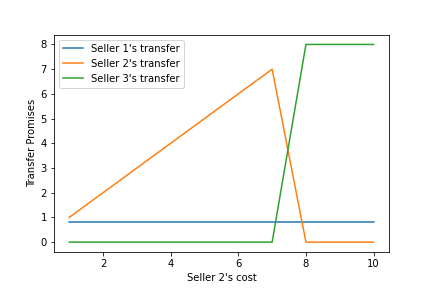
\includegraphics[width=0.8\textwidth]{\FigDir/sampleTP.png}}
	\caption{Sellers' payments under Transfer Promises}
	\label{fig:sampleTP}
\end{figure}	
\end{frame}

\begin{frame}[shrink = 5]
	\frametitle{Comparison of Two Payment Methods}
	\hypertarget{sampleTP}{}
\begin{figure}
	\centerline{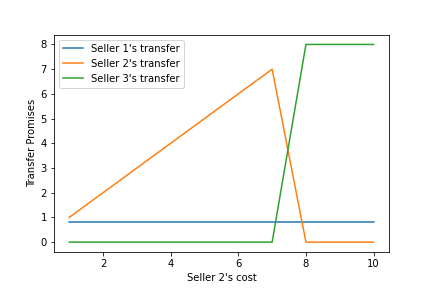
\includegraphics[width=0.8\textwidth]{\FigDir/sampleTP.png}}
	\caption{Sellers' payments under Transfer Promises}
	\label{fig:sampleTP}
\end{figure}
\end{frame}

\section{Extension}
\begin{frame}
	\frametitle{2nd-year Paper}
	In my second-year paper, I plan to extend the Chen-Zapal model by adding in the formation of coalition as an extra stage before the actual bargaining.
	The main focus, rather than considering the best sequencing, would be rationalize the coalition formation behavior. 
\end{frame}


\def\newblock{\hskip .11em plus .33em minus .07em}

\begin{frame}

\renewcommand{\bibsection}{\subsubsection*{\bibname }}

\tiny 

\bibliography{\texnameMaster,\econtexBib}

\end{frame}
\end{document}\endinput

% Local Variables:
% eval: (setq TeX-command-list  (remove '("Biber" "biber %s" TeX-run-Biber nil  (plain-tex-mode latex-mode doctex-mode ams-tex-mode texinfo-mode)  :help "Run Biber") TeX-command-list))
% eval: (setq TeX-command-list  (remove '("BibTeX" "%(bibtex) %s" TeX-run-BibTeX nil t                                                                              :help "Run BibTeX") TeX-command-list))
% eval: (setq TeX-command-list  (remove '("BibTeX" "%(bibtex) %s" TeX-run-BibTeX nil (plain-tex-mode latex-mode doctex-mode ams-tex-mode texinfo-mode context-mode) :help "Run BibTeX") TeX-command-list))
% eval: (setq TeX-command-list  (remove '("BibTeX" "%(bibtex) ../LaTeX/%s" TeX-run-BibTeX nil t :help "Run BibTeX")   TeX-command-list))
% eval: (add-to-list 'TeX-command-list	'("BibTeX" "%(bibtex) LaTeX/%s" TeX-run-BibTeX nil t :help "Run BibTeX") t)
% eval: (cond ((string-equal system-type "darwin") (progn (setq TeX-view-program-list '(("Skim" "/Applications/Skim.app/Contents/SharedSupport/displayline -b %n LaTeX/%o %b"))))))
% TeX-PDF-mode: t
% TeX-file-line-error: t
% TeX-debug-warnings: t
% LaTeX-command-style: (("" "%(PDF)%(latex) %(file-line-error) %(extraopts) -output-directory=LaTeX %S%(PDFout)"))
% TeX-source-correlate-mode: t
% TeX-source-correlate-start-server: 0
% TeX-parse-self: t
% End:
